\documentclass{article}

\usepackage[english]{babel}
\usepackage{blindtext}

\title{An EPS trimming workflow}
\author{Brandon Barker}
\date{\today}

\usepackage{caption}
\usepackage{graphicx}
\usepackage{subcaption}
\usepackage{float}


\begin{document}

% Let's draw a box around the figure so we
% can see where the figure's whitespace ends.
\setlength\fboxsep{0pt}
\setlength\fboxrule{1.5pt}

\begin{figure}[h] 
\centering
% give some space for fbox:                    % l       b   r   t
\fbox{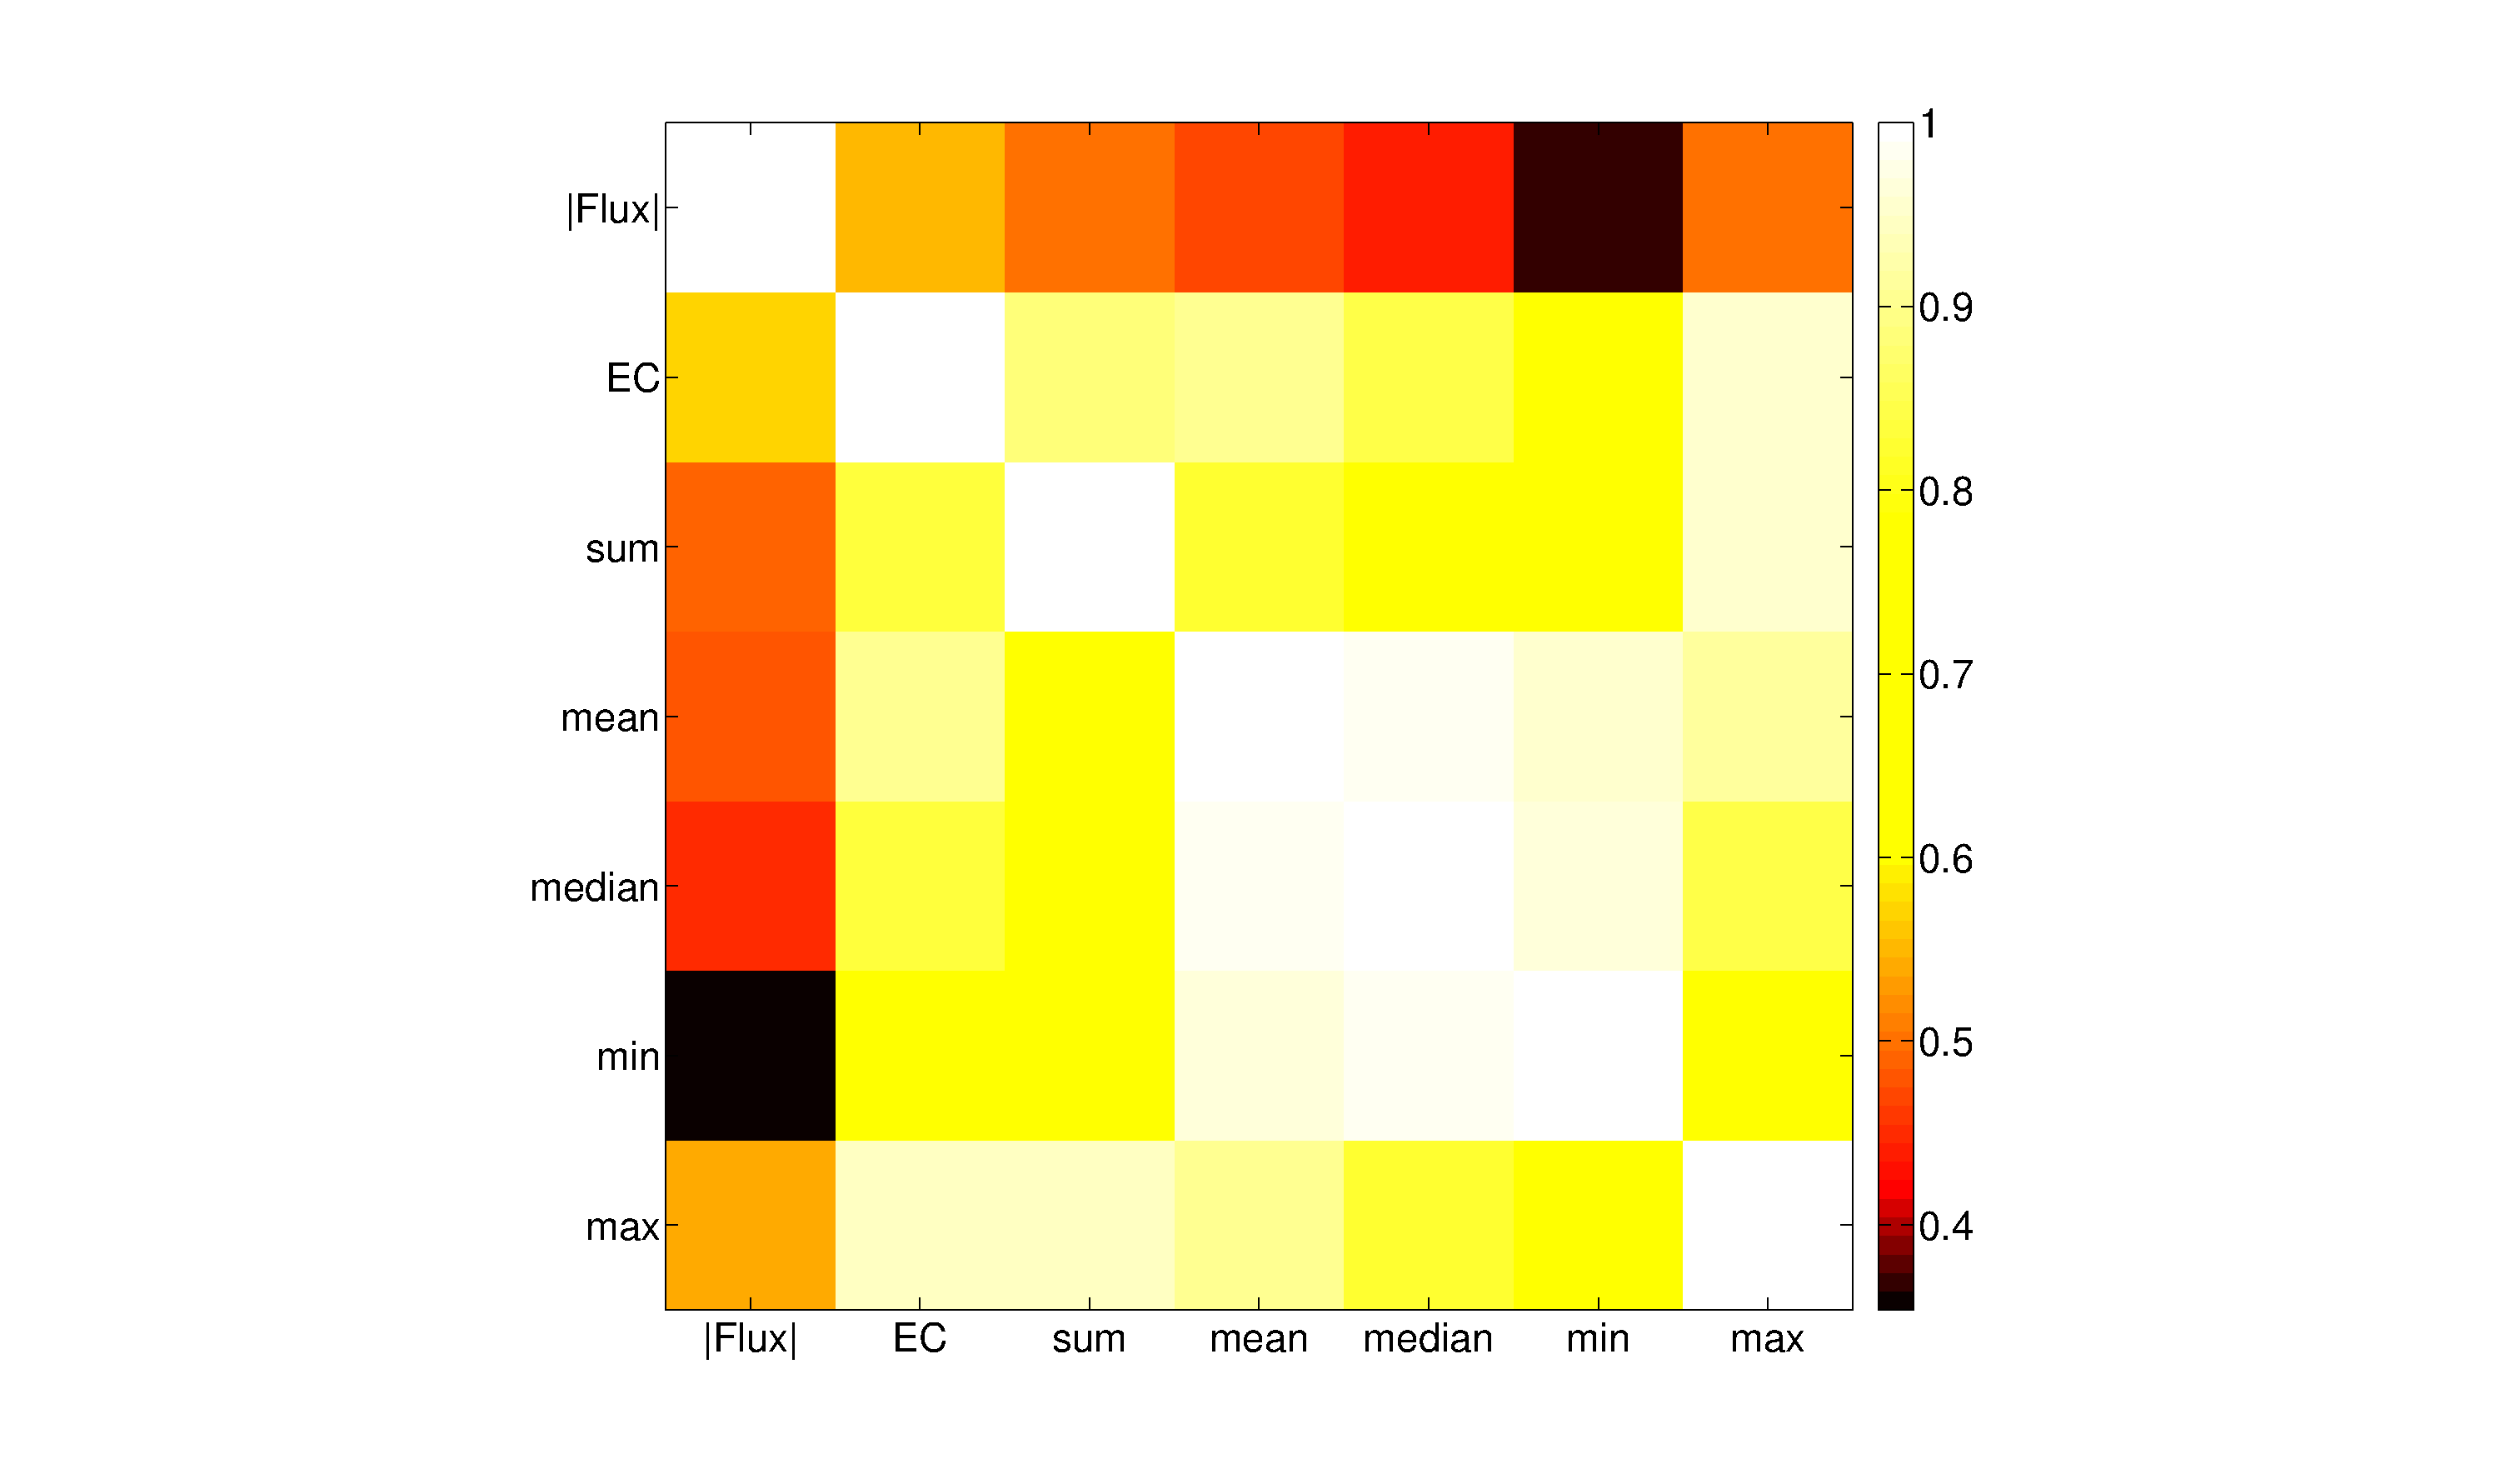
\includegraphics[width=0.9\textwidth, trim=104.4mm 0mm 0mm 17.3mm, clip=true]
      {YeastExpFluxCompare}}
\caption{\blindtext}
\label{fig:FluxExpCmp}
\end{figure}

Please refer to Table~\ref{fig:FluxExpCmp}.

\end{document}
